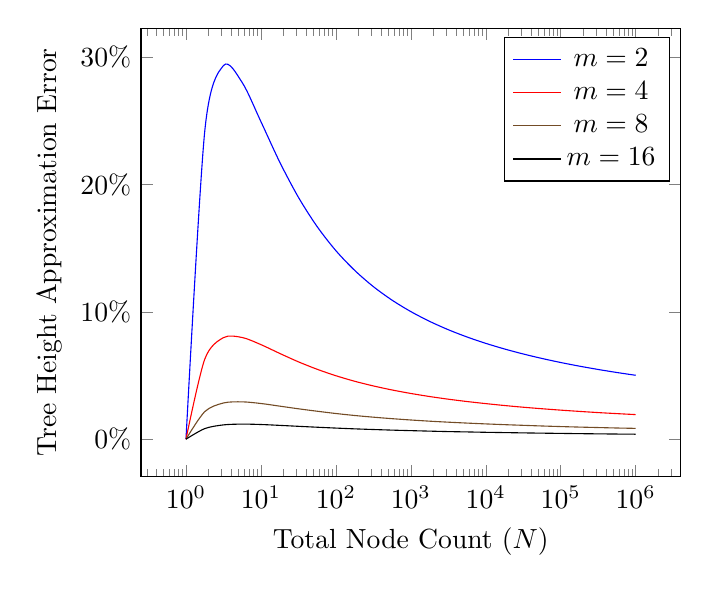
\begin{tikzpicture}
	\begin{axis}
		[
			xlabel={Total Node Count ($N$)},
			ylabel={Tree Height Approximation Error},
			domain=1:1000000,
			xmode=log,
			yticklabel={%
				\pgfmathparse{\tick*100}%
				\pgfmathprintnumber{\pgfmathresult}%
				\%%
			},
			smooth
		]
		\pgfplotsinvokeforeach{2,4,8,16} {
			\addplot+[cycle list name=color list, mark=none]
				{
					(
						(
							1+ln(x)/ln(#1)
						) - (
							ln(1 - x*(1-#1)) / ln(#1)
						)
					) / (
						ln(1 - x*(1-#1)) / ln(#1)
					)
				};
			\addlegendentry{$m=#1$}
		}
	\end{axis}
\end{tikzpicture}
